\documentclass[12pt,a4paper]{article}
\usepackage{amsmath} % For advanced math formatting
\usepackage{enumitem} % For customising lists
\usepackage{tikz} % For drawing diagrams
\usepackage{geometry} % For adjusting page margins
\geometry{margin=1in}


\title{Ratio Extension Problems}
\date{}

\begin{document}


\maketitle

\section*{Simplifying Ratios Past}
\emph{Simplify the following ratios. Some questions involve working with percentages first.}

\begin{enumerate}
\item In a survey, 60\% of people preferred tea and 40\% preferred coffee. Write the ratio of tea drinkers to coffee drinkers in its simplest form.

\vspace{1.2cm}

\item A shirt is on sale for 30\% off. The discount amount is £12. What is the ratio of the discount amount to the original price? Simplify your answer.

\vspace{1.2cm}

\item A battery has lost 15\% of its charge. What is the ratio of the charge lost to the charge remaining? Simplify your answer.

\vspace{1.2cm}

\item In a year, a company's profits were allocated as follows: 45\% was reinvested, 20\% was paid as dividends, and the rest was used for employee bonuses.
    \begin{enumerate}
    \item What percentage was used for employee bonuses?
    \item Express the ratio Reinvestment : Dividends : Bonuses in its simplest form.
    \end{enumerate}

\vspace{1.2cm}

\item The population of a town is 12,500. After a census, it's found that the population has increased by 18\%. What is the ratio of the new population to the original population? Express your answer in the form \( a : b \), where \( a \) and \( b \) are integers.

\end{enumerate}

\newpage{}

\section*{Simplifying Ratios Future}
\emph{Use the diagrams to help you answer the questions about the ratios of areas and perimeters.}

\begin{enumerate}
\setcounter{enumi}{5}
\item The two rectangles below are similar. Find the ratio of the perimeter of rectangle A to the perimeter of rectangle B. Then, find the ratio of the area of rectangle A to the area of rectangle B.

\vspace{0.5cm}
\begin{center}
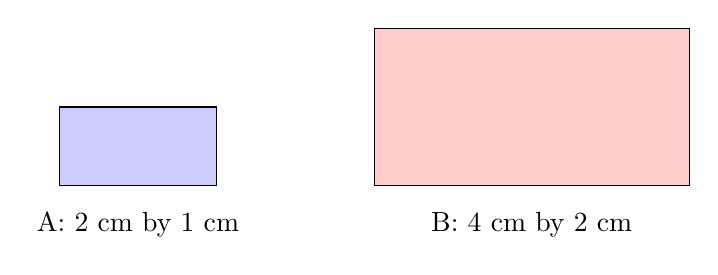
\begin{tikzpicture}
\draw[fill=blue!20] (0,0) rectangle (2,1);
\node at (1, -0.5) {A: 2 cm by 1 cm};
\draw[fill=red!20] (4,0) rectangle (8,2);
\node at (6, -0.5) {B: 4 cm by 2 cm};
\end{tikzpicture}
\end{center}

\vspace{1.2cm}

\item A square has a side length of \( s \). Another square has a side length of \( 3s \). What is the ratio of the perimeter of the smaller square to the larger square? What is the ratio of their areas?

\vspace{1.2cm}

\item A right-angled triangle has a base of 8 cm and a height of 6 cm. A similar triangle has a base of 12 cm.
    \begin{enumerate}
    \item What is the scale factor from the smaller to the larger triangle?
    \item What is the ratio of the perimeter of the smaller triangle to the larger triangle?
    \item What is the ratio of the area of the smaller triangle to the larger triangle?
    \end{enumerate}

\vspace{1.2cm}

\newpage{}

\item The diagram below shows a large rectangle with a smaller rectangle cut out of it. Find the ratio of the area of the shaded region to the area of the unshaded (cut-out) rectangle.

\vspace{0.5cm}
\begin{center}
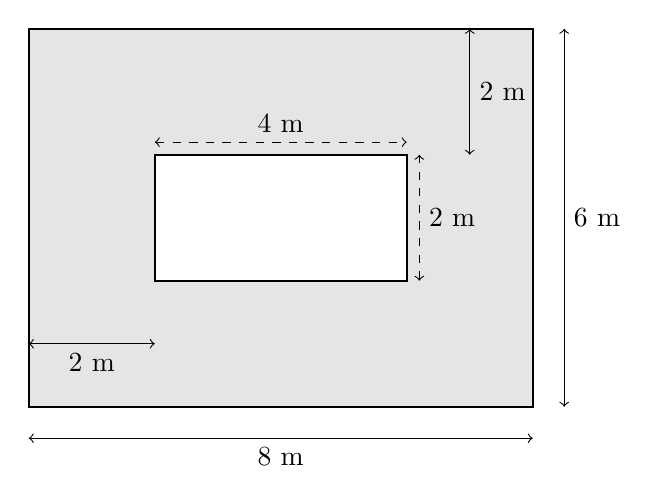
\begin{tikzpicture}[scale=0.8]
    % Big rectangle (shaded region)
    \fill[gray!20] (0,0) rectangle (8,6);
    \draw[thick] (0,0) rectangle (8,6);
    
    % Small rectangle (cut-out) - drawn with thicker white border to show cut-out effect
    \fill[white] (2,2) rectangle (6,4);
    \draw[thick, white] (2,2) rectangle (6,4);
    \draw[thick] (2,2) rectangle (6,4);
    
    % Labels for dimensions
    % Outer rectangle dimensions
    \draw[<->] (0,-0.5) -- (8,-0.5) node[midway,below] {8 m};
    \draw[<->] (8.5,0) -- (8.5,6) node[midway,right] {6 m};
    
    % Inner rectangle positioning dimensions
    \draw[<->] (0,1) -- (2,1) node[midway,below] {2 m};
    \draw[<->] (7,4) -- (7,6) node[midway,right] {2 m};
    
       
    % Inner rectangle dimensions
    \draw[<->, dashed] (2,4.2) -- (6,4.2) node[midway,above] {4 m};
    \draw[<->, dashed] (6.2,2) -- (6.2,4) node[midway,right] {2 m};
\end{tikzpicture}
\end{center}
\textit{(Dimensions: Large rectangle is 8m by 6m. The unshaded rectangle has a length of 4m and is positioned centrally.)}

\vspace{1.2cm}

\item A circular pond has a radius of \( r \). A path is built around it, creating a larger circle with a radius of \( R \), where \( R = 2r \).
    \begin{enumerate}
    \item Find the ratio of the circumference of the pond to the circumference of the outer edge of the path.
    \item Find the ratio of the area of the pond to the total area enclosed by the outer edge of the path.
    \end{enumerate}

\vspace{1.2cm}
\end{enumerate}

\section*{Sharing Into Ratios Past}
Share the given quantities in the specified ratios, using the percentage information to help you.

\begin{enumerate}
    \setcounter{enumi}{10}
    \item A sum of £80 is shared between two people. Person A receives 60\% of the total. What is the ratio of their shares, and how much does each person receive?

    \item In a class, 40\% of students are boys and the rest are girls. The school fund of £150 is to be shared between boys and girls in the same ratio as their numbers in the class. How much do the boys get?
    
    \item A bonus of £2,500 is shared between three departments in proportion to their percentage contribution to company profits. Department A contributed 25\%, Department B 35\%, and Department C the remainder. How much does each department receive, and what is the ratio of their shares in simplest form?
    
    \item In a recipe, the dry ingredients (flour and sugar) are mixed in the ratio 3:2 by weight. If the flour makes up 30\% of the total mixture (including 400g of wet ingredients), find the weight of flour and sugar used.
    
    \item An inheritance is shared between three children. The eldest receives 50\% of the total, the middle child receives 40\% of what the eldest gets, and the youngest receives the remaining £24,000. Find the total inheritance and the ratio of their shares in the form \textit{Eldest : Middle : Youngest}.
\end{enumerate}



\section*{Sharing Into Ratios Future}
Use the diagrams to help you solve the following problems.

\begin{enumerate}
    \setcounter{enumi}{15}
    \item The perimeter of a rectangle is 30 cm. The sides are in the ratio 2:3. Find the area of the rectangle.
    
    \item The area of a rectangle is 54 cm². The sides are in the ratio 2:3. Find the perimeter of the rectangle.
    

    \item A right-angled triangle has sides in the ratio 3:4:5. The area of the triangle is 96 cm². Find the perimeter of the triangle.
    
    \begin{tikzpicture}
        \draw (0,0) -- (4,0) -- (0,3) -- cycle;
        \node at (2, -0.3) {?};
        \node at (-0.3, 1.5) {?};
        \node at (2, 1.8) {?};
    \end{tikzpicture}

    \item A garden is in the shape of an L-shape made from two rectangles. The first rectangle is 3m by 2m. The second rectangle has sides in the ratio 3:4, If the total area of the garden is 54 m², find the dimensions of the second rectangle.
    
    \begin{tikzpicture}[scale=0.5]
        \draw (0,0) rectangle (3,2);
        \draw (3,0) rectangle (7,4);
        \node at (1.5, -0.5) {3m};
        \node at (-0.55, 1) {2m};
        \node at (5, -0.5) {?};
        \node at (8, 2) {?};
    \end{tikzpicture}

    \newpage{}

    \item A circular pond is surrounded by a path. The radius of the pond and the width of the path are in the ratio 2:1. If the total area (pond + path) is $99\pi$m², find the width of the path.
    
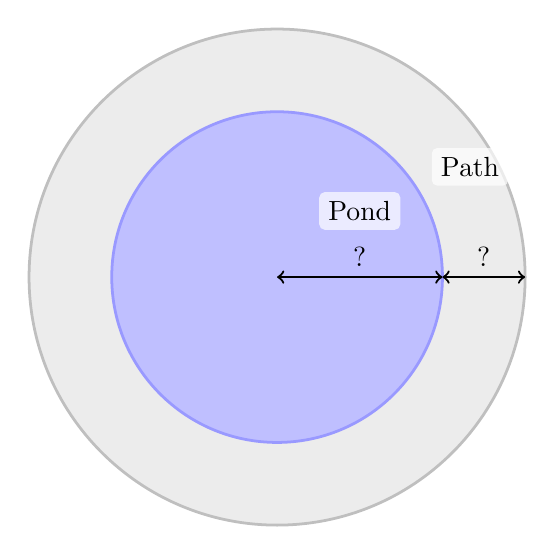
\begin{tikzpicture}[scale=0.7]
    % Path (annulus) - lighter fill with darker border
    \filldraw[fill=gray!15, draw=gray!50, line width=1pt] (0,0) circle (4.5);
    % Pond - darker fill with clear border
    \filldraw[fill=blue!25, draw=blue!40, line width=1pt] (0,0) circle (3);
    
    % Dimension lines with arrows and labels
    \draw[<->, line width=0.8pt] (0,0) -- (3,0) node[midway, above]{?};
    \draw[<->, line width=0.8pt] (3,0) -- (4.5,0) node[midway, above] {?};
    
    % Labels with better positioning and background
    \node[fill=white, fill opacity=0.7, text opacity=1, rounded corners=2pt] at (1.5, 1.2) {Pond};
    \node[fill=white, fill opacity=0.7, text opacity=1, rounded corners=2pt] at (3.5, 2.0) {Path};
    
\end{tikzpicture}
\end{enumerate}

\vspace{1cm}

\section*{Ratio Problem Solving Past}
\begin{enumerate}[start=21]

    \item In a class, the ratio of boys to girls is $3:2$. 40\% of the boys wear glasses. 20\% of the girls wear glasses, what percentage of the \textit{whole class} wear glasses?

    \item The price of a rare coin is increased by 20\%. The new ratio of its price to its original price is $a : b$. Write the ratio $a:b$ in its simplest form.

    \item A shop sells only two types of fruit: apples and oranges. The ratio of apples to oranges is $5:3$. 30\% of the apples are green, and the rest are red. 60\% of the oranges are from Spain, and the rest are from Morocco. What is the ratio of \textbf{green apples} to \textbf{oranges from Morocco}?

    \item In a library, the ratio of fiction to non-fiction books is $7:3$. After a donation, the number of fiction books increased by 15\% and the number of non-fiction books decreased by 10\%. Find the new ratio of fiction to non-fiction books. Give your answer in the form $A:B$ where $A$ and $B$ are integers.

    \item The population of a town is 18,000. The ratio of adults to children is $5:4$. One year later, the adult population decreases by 5\% and the child population increases by 10\%.
    \begin{enumerate}[label=(\alph*)]
        \item What is the new ratio of adults to children? Give your answer in its simplest form.
        \item What is the overall percentage change in the total population? Give your answer to 2 decimal places.
    \end{enumerate}

\end{enumerate}

\newpage{}


\section*{Ratio Problem Solving Future}
\begin{enumerate}[start=26]

    \item Two rectangles, A and B, are similar. The ratio of their corresponding lengths is $2:5$. What is the ratio of their perimeters? What is the ratio of their areas?

    \item A rectangle has a length to width ratio of $5:2$. Its perimeter is 42 cm.
    \begin{enumerate}[label=(\alph*)]
        \item Find its area.
        \item If the rectangle is enlarged by a scale factor of 3, what is the new ratio of length to width, and what is its new area?
    \end{enumerate}

    \item The ratio of the area of a square to the area of an equilateral triangle is $16:9$. The perimeter of the square is 32 cm. What is the length of one side of the triangle?

    \item The perimeter of an isosceles triangle is 36 cm. The ratio of the equal sides to the base is $5:2$.
    \begin{enumerate}[label=(\alph*)]
        \item Calculate the lengths of the sides of the triangle.
        \item Calculate the area of the triangle. (Hint: You may need to use Pythagoras' Theorem - ask your teacher to help you draw a picture!).
    \end{enumerate}

    \item The diagram below shows a large rectangle, measuring 20 cm at the base, with a similar smaller rectangle, height 4 cm cut out from one corner. The ratio of the length to the width of the smaller rectangle is the same as the ratio of the length to the width of the large rectangle.
    
    \begin{center}
    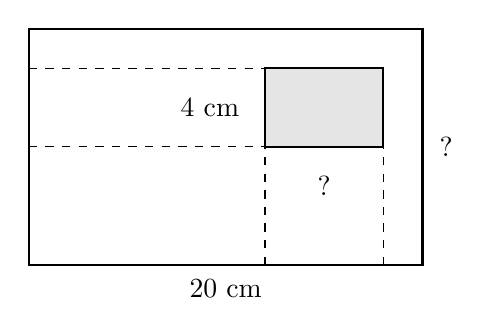
\begin{tikzpicture}
        \draw[thick] (0,0) rectangle (5,3);
        \draw[thick, fill=gray!20] (3,1.5) rectangle (4.5,2.5);
        \draw[dashed] (3,0) -- (3,1.5);
        \draw[dashed] (4.5,0) -- (4.5,1.5);
        \draw[dashed] (0,1.5) -- (3,1.5);
        \draw[dashed] (0,2.5) -- (3,2.5);
        \node at (2.5, -0.3) {20 cm};
        \node at (5.3, 1.5) {?};
        \node at (2.3, 2) {4 cm};
        \node at (3.75, 1) {?};
    \end{tikzpicture}
    \end{center}
    
    Given that the area of the large rectangle with the small one cut out is $216 \text{ cm}^2$, find the dimensions of the smaller rectangle.

\end{enumerate}

\end{document}
